\documentclass[border=6pt,tikz]{standalone}
\usepackage{tikz}
\usepackage{amsmath,amssymb}
\usetikzlibrary{arrows.meta,positioning,fit,backgrounds,calc,shapes.geometric,decorations.pathreplacing,patterns}
\definecolor{ink}{HTML}{1B2430}
\definecolor{muted}{HTML}{6B7785}
\definecolor{accent}{HTML}{2F6FB5}
\definecolor{accent2}{HTML}{C1611F}
\definecolor{good}{HTML}{2E7D5B}
\definecolor{soft}{HTML}{EDF2F7}
\definecolor{soft2}{HTML}{FBEDE2}
\definecolor{soft3}{HTML}{E6F0E9}
\tikzset{
  box/.style={draw=ink,line width=.7pt,rounded corners=2pt,fill=soft,inner sep=4pt,align=center,font=\sffamily\small},
  boxa/.style={box,fill=soft2},
  boxb/.style={box,fill=soft3},
  plain/.style={align=center,font=\sffamily\small,text=ink},
  tiny/.style={align=center,font=\sffamily\scriptsize,text=muted},
  ar/.style={-{Stealth[length=2.4mm]},draw=ink,line width=.7pt},
  arm/.style={-{Stealth[length=2.4mm]},draw=muted,line width=.6pt,dashed},
  nd/.style={circle,draw=ink,line width=.7pt,fill=white,minimum size=7mm,inner sep=0pt,font=\sffamily\scriptsize},
  ndf/.style={nd,fill=soft},
  ndt/.style={nd,fill=soft2},
}

\begin{document}
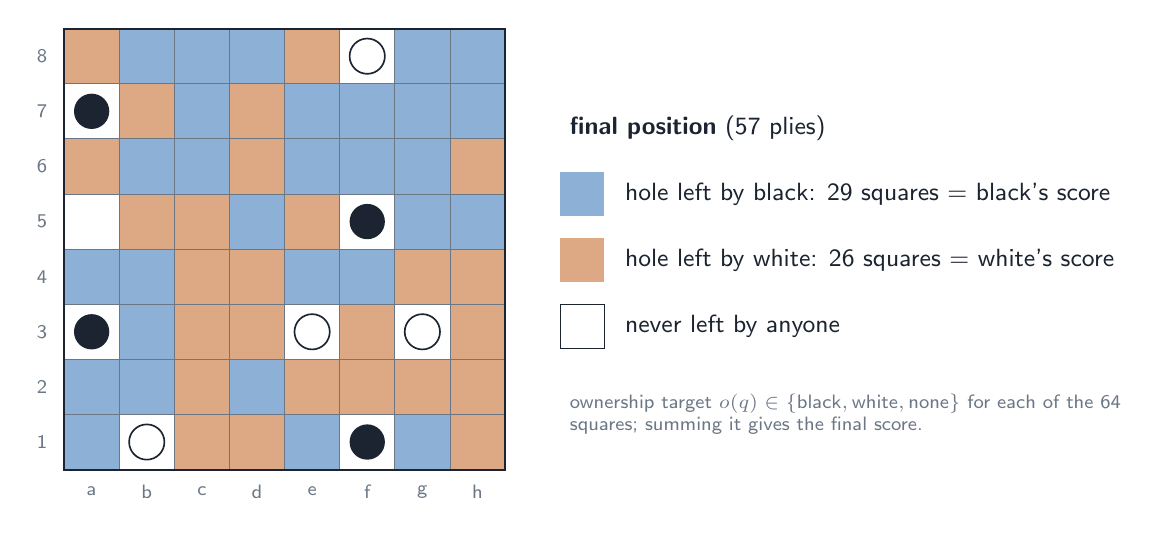
\begin{tikzpicture}[x=7mm,y=7mm]
\fill[accent!55] (0,0) rectangle ++(1,1);
\fill[white] (1,0) rectangle ++(1,1);
\fill[accent2!55] (2,0) rectangle ++(1,1);
\fill[accent2!55] (3,0) rectangle ++(1,1);
\fill[accent!55] (4,0) rectangle ++(1,1);
\fill[white] (5,0) rectangle ++(1,1);
\fill[accent!55] (6,0) rectangle ++(1,1);
\fill[accent2!55] (7,0) rectangle ++(1,1);
\fill[accent!55] (0,1) rectangle ++(1,1);
\fill[accent!55] (1,1) rectangle ++(1,1);
\fill[accent2!55] (2,1) rectangle ++(1,1);
\fill[accent!55] (3,1) rectangle ++(1,1);
\fill[accent2!55] (4,1) rectangle ++(1,1);
\fill[accent2!55] (5,1) rectangle ++(1,1);
\fill[accent2!55] (6,1) rectangle ++(1,1);
\fill[accent2!55] (7,1) rectangle ++(1,1);
\fill[white] (0,2) rectangle ++(1,1);
\fill[accent!55] (1,2) rectangle ++(1,1);
\fill[accent2!55] (2,2) rectangle ++(1,1);
\fill[accent2!55] (3,2) rectangle ++(1,1);
\fill[white] (4,2) rectangle ++(1,1);
\fill[accent2!55] (5,2) rectangle ++(1,1);
\fill[white] (6,2) rectangle ++(1,1);
\fill[accent2!55] (7,2) rectangle ++(1,1);
\fill[accent!55] (0,3) rectangle ++(1,1);
\fill[accent!55] (1,3) rectangle ++(1,1);
\fill[accent2!55] (2,3) rectangle ++(1,1);
\fill[accent2!55] (3,3) rectangle ++(1,1);
\fill[accent!55] (4,3) rectangle ++(1,1);
\fill[accent!55] (5,3) rectangle ++(1,1);
\fill[accent2!55] (6,3) rectangle ++(1,1);
\fill[accent2!55] (7,3) rectangle ++(1,1);
\fill[white] (0,4) rectangle ++(1,1);
\fill[accent2!55] (1,4) rectangle ++(1,1);
\fill[accent2!55] (2,4) rectangle ++(1,1);
\fill[accent!55] (3,4) rectangle ++(1,1);
\fill[accent2!55] (4,4) rectangle ++(1,1);
\fill[white] (5,4) rectangle ++(1,1);
\fill[accent!55] (6,4) rectangle ++(1,1);
\fill[accent!55] (7,4) rectangle ++(1,1);
\fill[accent2!55] (0,5) rectangle ++(1,1);
\fill[accent!55] (1,5) rectangle ++(1,1);
\fill[accent!55] (2,5) rectangle ++(1,1);
\fill[accent2!55] (3,5) rectangle ++(1,1);
\fill[accent!55] (4,5) rectangle ++(1,1);
\fill[accent!55] (5,5) rectangle ++(1,1);
\fill[accent!55] (6,5) rectangle ++(1,1);
\fill[accent2!55] (7,5) rectangle ++(1,1);
\fill[white] (0,6) rectangle ++(1,1);
\fill[accent2!55] (1,6) rectangle ++(1,1);
\fill[accent!55] (2,6) rectangle ++(1,1);
\fill[accent2!55] (3,6) rectangle ++(1,1);
\fill[accent!55] (4,6) rectangle ++(1,1);
\fill[accent!55] (5,6) rectangle ++(1,1);
\fill[accent!55] (6,6) rectangle ++(1,1);
\fill[accent!55] (7,6) rectangle ++(1,1);
\fill[accent2!55] (0,7) rectangle ++(1,1);
\fill[accent!55] (1,7) rectangle ++(1,1);
\fill[accent!55] (2,7) rectangle ++(1,1);
\fill[accent!55] (3,7) rectangle ++(1,1);
\fill[accent2!55] (4,7) rectangle ++(1,1);
\fill[white] (5,7) rectangle ++(1,1);
\fill[accent!55] (6,7) rectangle ++(1,1);
\fill[accent!55] (7,7) rectangle ++(1,1);
\draw[muted,line width=.3pt] (0,0) grid[step=1] (8,8); \draw[ink,line width=.7pt] (0,0) rectangle (8,8);
\filldraw[fill=white,draw=ink,line width=.6pt] (5.5,7.5) circle (.32);
\filldraw[fill=white,draw=ink,line width=.6pt] (1.5,0.5) circle (.32);
\filldraw[fill=white,draw=ink,line width=.6pt] (6.5,2.5) circle (.32);
\fill[ink] (0.5,6.5) circle (.32);
\filldraw[fill=white,draw=ink,line width=.6pt] (4.5,2.5) circle (.32);
\fill[ink] (5.5,4.5) circle (.32);
\fill[ink] (5.5,0.5) circle (.32);
\fill[ink] (0.5,2.5) circle (.32);
\node[tiny] at (0.5,-.4) {a};
\node[tiny] at (1.5,-.4) {b};
\node[tiny] at (2.5,-.4) {c};
\node[tiny] at (3.5,-.4) {d};
\node[tiny] at (4.5,-.4) {e};
\node[tiny] at (5.5,-.4) {f};
\node[tiny] at (6.5,-.4) {g};
\node[tiny] at (7.5,-.4) {h};
\node[tiny] at (-.4,0.5) {1};
\node[tiny] at (-.4,1.5) {2};
\node[tiny] at (-.4,2.5) {3};
\node[tiny] at (-.4,3.5) {4};
\node[tiny] at (-.4,4.5) {5};
\node[tiny] at (-.4,5.5) {6};
\node[tiny] at (-.4,6.5) {7};
\node[tiny] at (-.4,7.5) {8};
\node[plain,anchor=west,align=left] at (9,6.2) {\textbf{final position} (57 plies)};
\fill[accent!55] (9,4.6) rectangle ++(.8,.8); \node[plain,anchor=west] at (10,5) {hole left by black: 29 squares $=$ black's score};
\fill[accent2!55] (9,3.4) rectangle ++(.8,.8); \node[plain,anchor=west] at (10,3.8) {hole left by white: 26 squares $=$ white's score};
\draw[ink] (9,2.2) rectangle ++(.8,.8); \node[plain,anchor=west] at (10,2.6) {never left by anyone};
\node[tiny,anchor=west,align=left,text width=70mm] at (9,1) {ownership target $o(q)\in\{\text{black},\text{white},\text{none}\}$ for each of the 64 squares; summing it gives the final score.};
\end{tikzpicture}
\end{document}
